%% 
%% Copyright 2007, 2008, 2009 Elsevier Ltd
%% 
%% This file is part of the 'Elsarticle Bundle'.
%% ---------------------------------------------
%% 
%% It may be distributed under the conditions of the LaTeX Project Public
%% License, either version 1.2 of this license or (at your option) any
%% later version.  The latest version of this license is in
%%    http://www.latex-project.org/lppl.txt
%% and version 1.2 or later is part of all distributions of LaTeX
%% version 1999/12/01 or later.
%% 
%% The list of all files belonging to the 'Elsarticle Bundle' is
%% given in the file `manifest.txt'.
%% 

%% Template article for Elsevier's document class `elsarticle'
%% with numbered style bibliographic references
%% SP 2008/03/01

 \documentclass[final,5p,times,twocolumn]{elsarticle}

%% Use the option review to obtain double line spacing


%% The amssymb package provides various useful mathematical symbols
\usepackage{amssymb}
%% The amsthm package provides extended theorem environments
\usepackage{amsthm}
\usepackage{amsmath}
\usepackage{subcaption}
\usepackage[canadian]{babel}
\usepackage[breaklinks,hidelinks]{hyperref} 
\usepackage{verbatim}
\usepackage{float}

%% The lineno packages adds line numbers. Start line numbering with
%% \begin{linenumbers}, end it with \end{linenumbers}. Or switch it on
%% for the whole article with \linenumbers.
%% \usepackage{lineno}

\journal{Computational Material Science}

\begin{document}


\begin{frontmatter}

%% Title, authors and addresses

%% use the tnoteref command within \title for footnotes;
%% use the tnotetext command for theassociated footnote;
%% use the fnref command within \author or \address for footnotes;
%% use the fntext command for theassociated footnote;
%% use the corref command within \author for corresponding author footnotes;
%% use the cortext command for theassociated footnote;
%% use the ead command for the email address,
%% and the form \ead[url] for the home page:
%% \title{Title\tnoteref{label1}}
%% \tnotetext[label1]{}
%% \author{Name\corref{cor1}\fnref{label2}}
%% \ead{email address}
%% \ead[url]{home page}
%% \fntext[label2]{}
%% \cortext[cor1]{}
%% \address{Address\fnref{label3}}
%% \fntext[label3]{}

\title{Lattice Matcher: A Tool for Computing Epitaxial Surface Net Matching}

%% use optional labels to link authors explicitly to addresses:
%% \author[label1,label2]{}
%% \address[label1]{}
%% \address[label2]{}

\author{Gabriel A. Devenyi}
\author{Stephen J. Smith}
\author{John S. Preston}

\address{Department of Engineering Physics, McMaster University, Hamilton, ON, Canada}

\begin{abstract}
%% Text of abstract

\end{abstract}

\begin{keyword}
%% keywords here, in the form: keyword \sep keyword

%% PACS codes here, in the form: \PACS code \sep code

%% MSC codes here, in the form: \MSC code \sep code
%% or \MSC[2008] code \sep code (2000 is the default)

\end{keyword}

\end{frontmatter}

%% \linenumbers

%% main text
\section{Introduction}
\label{Introduction}
The lattice match (or it’s compliment, mismatch) between two crystal is a central concept in the field of epitaxial growth. It is most commonly defined as in Equation~\ref{eqn:mismatch}, and is conceived of as the difference between the lattice constants of two cubes, sharing an interface that consists of their (001) faces. Such a expression of the lattice match has been very successful at predicting heteroepitaxial crystal matches of technological relevance, most importantly the III-V binary semiconductor systems. Such a definition has also be very successful at modelling changes to band structure\cite{Chuang1991}, growth modes\cite{Dunstan1997} and strain\cite{Dunstan1997}.
\begin{equation}
\text{mismatch} = 1 - \frac{a_f}{a_s} \label{eqn:mismatch}
\end{equation}

There have been several extensions made to the basic ideas of epitaxy, Palmstrom et al. \cite{Palmstrom1995} presented a model of epitaxial mismatch which noted both that sub- and super-lattice (integer ratio of lattice parameters) and rotation of in-plane cubes allows addition lattice matches between materials. Narayan et al. \cite{Narayan2003} presented a concept of epitaxial matching they coined “Domain epitaxy” where lattice matching is achieved when ratios of film to substrate lattice spacing coincide periodically, such as 4 film lattice parameters for every 3 substrate lattice parameters, providing the ratio 4/3. In both cases the authors rely on the fact that the symmetry between the film and substrate are the same, or the relationship is “similar.”

In this work, we present an alternate epitaxial model called ``surface net matching.'' In this model of epitaxial matching, matches are expressed via the alignment of two dimensional nets projected onto the epitaxial interface. This allows for new types of epitaxial matches, as two dimensional projections of lattices can have different symmetries than the bulk, such as for cubic crystals where (001) is 4-fold, (111) is 3-fold and (011) is 2-fold. Under this model, we derive and present several new lattice match conditions for cubic, tetragonal, and hexagonal material systems. Matching projected two dimensional nets reveals epitaxial matches between materials from different crystal systems that may have technological relevance. The ideas behind this model and software have been used to investigate a number of new heteroepitaxial growth systems \cite{Devenyi2009,Neretina2006,Neretina2008b}.

In addition to presenting the net matching model of epitaxy, we have developed a general purpose computer program for computing the matches predicted by this model, for a user provided database of materials and specified tolerance. A program is also provided to compute the net matching for arbitrary compositions of multicomponent systems, with the III-V quaternary system provided for reference.

\section{Theory}
The first extension of the lattice match equation is the introduction of the sub- and super-lattice matching from Palmstrom. The sub and super-lattice extension is implemented into the general definition of the cubic lattice mismatch equation (Equation~\ref{eqn:mismatch}), through the addition of the ratio parameter ($r$), resulting in Equation~\ref{eqn:mismatch_ratio}. The ratio parameter is a positive integer (2,3,4 etc) or fraction (1/2, 1/3, 1/4, etc) which scales the lattice parameter of the film to be closest to that of the substrate. This ratio parameter is the number of unit cells of the film that will pattern the substrate.
\begin{equation}
\text{mismatch} = 1 - r \frac{a_f}{a_s} \label{eqn:mismatch_ratio}
\end{equation}

The second extension of the lattice mismatch equation is the introduction of 2D surface nets. The 2D surface net is a construction formed by slicing through various high symmetry (low index) miller indices of 3D crystal lattices, resulting in a 2D projection of the 3D lattice. These 2D projections have different symmetry than the 3D lattice, revealing new symmetry matches between films and substrates. This is most clearly illustrated by high symmetry cuts through cubic crystals, as shown in Figure~\ref{fig:cubic_planes}. A cubic crystal cut along a cube face \{001\}, presents a square 2D surface net, cut along {011} presents a rectangular 2D surface net (side length $\sqrt(2)a$), and cut along \{111\} presents a triangular surface net (side length $\sqrt(2)a$). This means that while we would typically consider a cubic crystal to have square-on-square lattice matches, it could also successfully tile substrates that present rectangular or triangular surface nets.
\begin{figure}
    \centering
\begin{subfigure}{0.3\textwidth}
    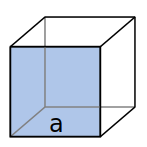
\includegraphics{graphics/cubic_010.pdf}
\end{subfigure}\quad
\begin{subfigure}{0.3\textwidth}
    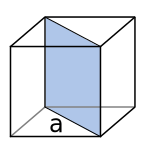
\includegraphics{graphics/cubic_110.pdf}
\end{subfigure}\quad
\begin{subfigure}{0.3\textwidth}
    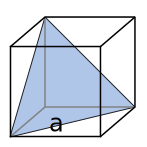
\includegraphics{graphics/cubic_111.pdf}
\end{subfigure}
    \caption{The three low index planes of cubic crystals a) (100) b) (110) and c) (111) \label{fig:cubic_planes}}
\end{figure}

The other primary crystal systems of interest for epitaxy are the tetragonal and hexagonal crystal systems. Again, depending up on the direction of the cut through the crystal, these systems present 2D surface nets with different symmetry.

For the tetragonal crystal system, cuts along (001) present a square 2D surface net, while cuts along (100) and (010) present rectangular symmetry, as shown in Figure~\ref{fig:tetra_planes}.
\begin{figure}
    \centering
    \begin{subfigure}{0.3\textwidth}
        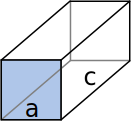
\includegraphics{graphics/base_tetragonal_original.pdf}
    \end{subfigure}\qquad
    \begin{subfigure}{0.3\textwidth}
        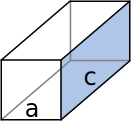
\includegraphics{graphics/tetragonal_a-plane.pdf}
    \end{subfigure}
    \caption{The two low index planes of tetragonal crystals a) (100) and b) (010) \label{fig:tetra_planes}}
\end{figure}

For the hexagonal crystal system, cuts along (0001) (c-plane) are typically interpreted as presenting 2D surface nets with hexagonal symmetry, however the 2D surface net also supports two equivalent orientations of triangular symmetry\cite{Neretina2009b}. Other cuts through the crystal (1120) (a-plane) and (1012) (r-plane) present rectangular 2D surface nets.
\begin{figure}
        \centering
        \begin{subfigure}{0.3\textwidth}
            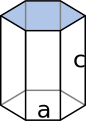
\includegraphics{graphics/hexagonal_0001.pdf}
        \end{subfigure}\quad
        \begin{subfigure}{0.3\textwidth}
            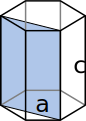
\includegraphics{graphics/hexagonal_a-plane.pdf}
        \end{subfigure}\quad
        \begin{subfigure}{0.3\textwidth}
            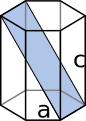
\includegraphics{graphics/hexagonal_r-plane.pdf}
        \end{subfigure}
    \caption{The three low index planes of hexagonal crystals a) (0001) b) a-plane c) r-plane \label{fig:hex_planes}}
\end{figure}

With the side lengths of each of the 2D surface nets now defined in terms of the original crystal lattice constants, and the definition of the lattice ratio parameter, we can now describe all of the possible symmetry-allowed lattice matches between cubic, tetragonal and hexagonal crystal systems, outlined in Figure~\ref{fig:match_matrix}.
\begin{figure*}
    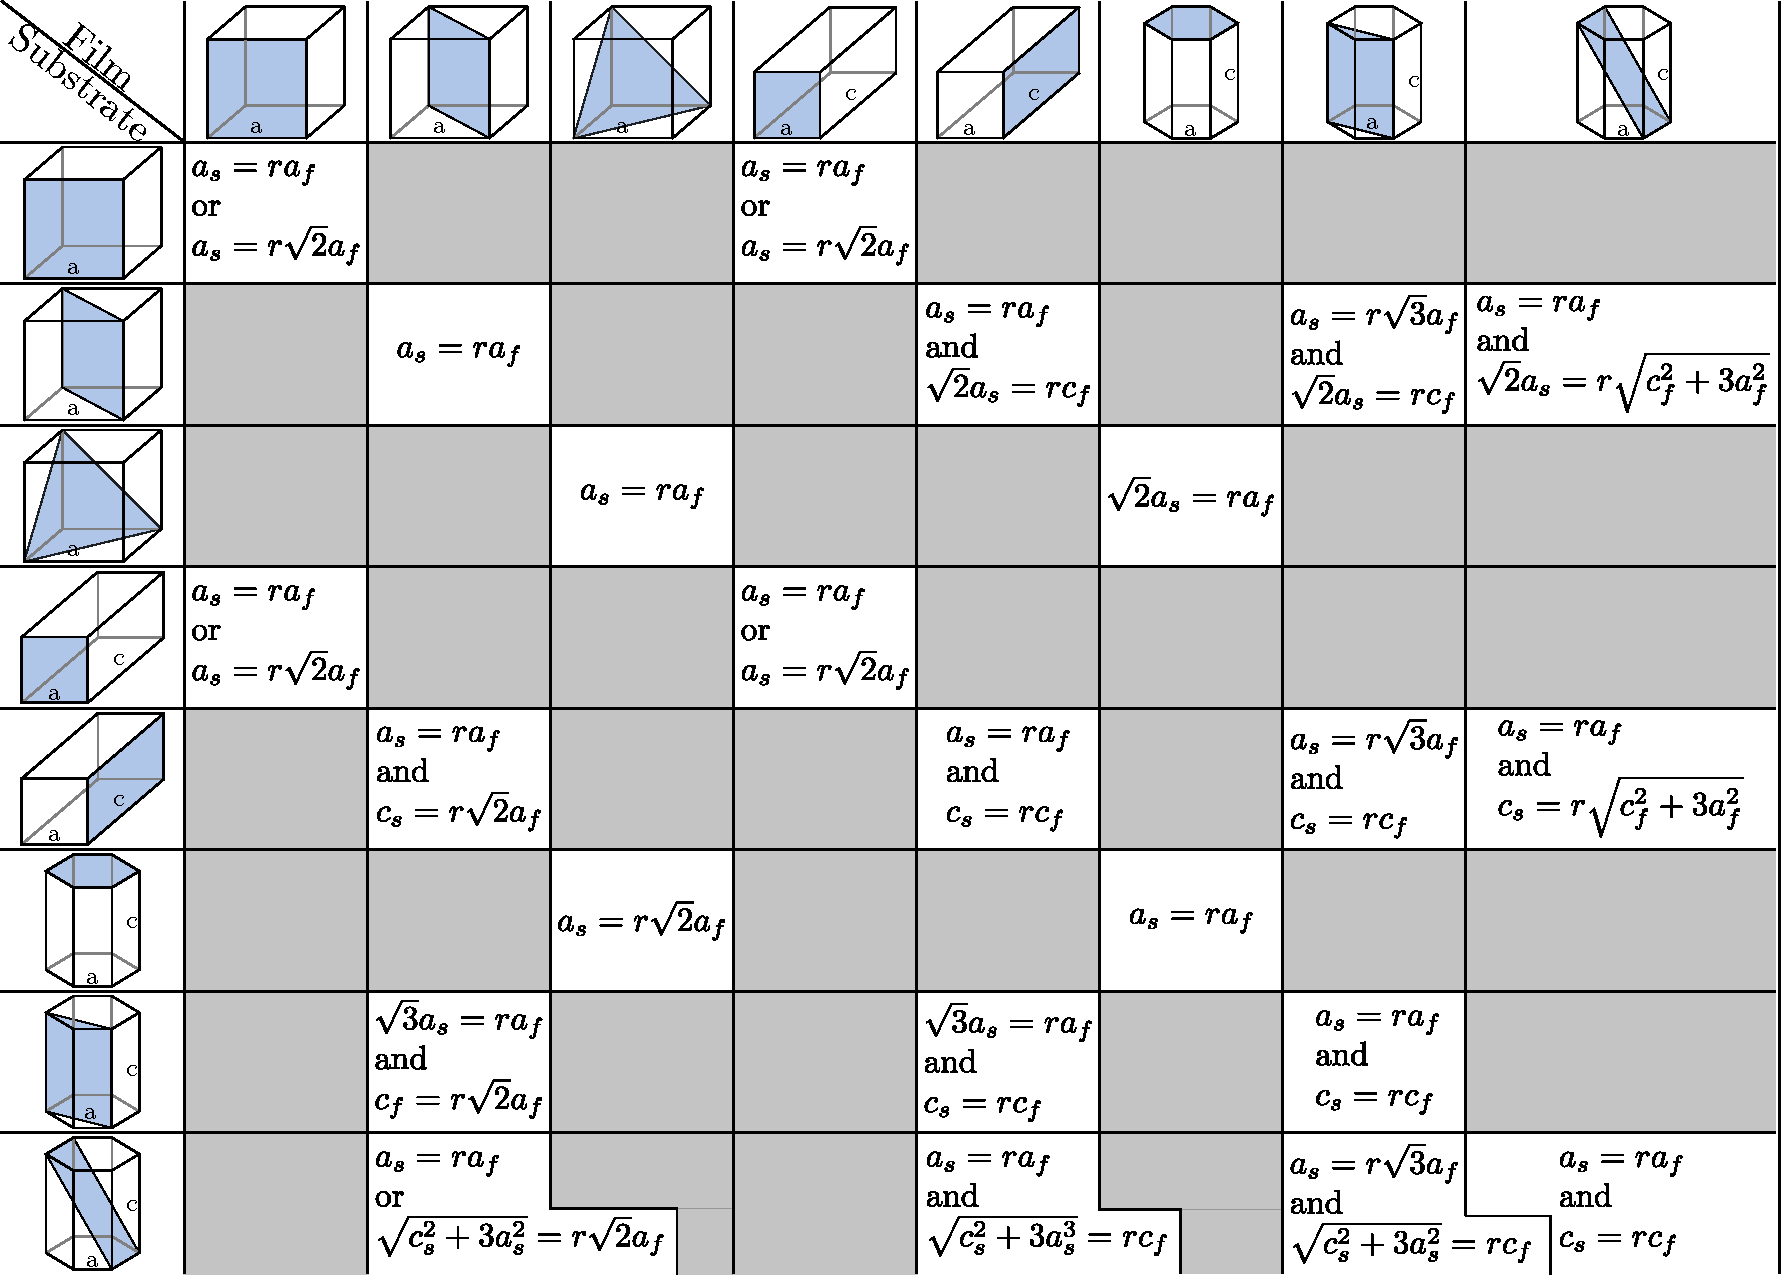
\includegraphics[width=\textwidth]{graphics/grid2.pdf}
    \caption{Lattice match between films ($a_f$) and substrates ($a_s$) computed using surface net matching\label{fig:match_matrix}}
\end{figure*}

In addition to the application of these lattice matching relationships to slices through bulk crystals, the surface net matching idea extends to the concept of surface reconstructions. There are numerous single crystals, particularly in the oxide family which form surface reconstructions on their exposed faces (through various combinations of annealing temperatures, atmospheres and surface crystal directions) that are stable at temperatures below their formation temperature, and possess different symmetries than their host crystal. These reconstructions present unique 2D surface nets which can host epitaxial crystals which typically would not match to the host crystal. This process is distinct from the intentional reconstructions performed on simple crystals such as silicon, as silicon reconstructions are destroyed by the formation of the growing epitaxial crystal. These stable surface reconstructions have been successfully used to influence the epitaxial growth of CdTe thin films on SrTiO3\cite{Neretina2009a}.

\section{Implementation}
In order to facilitate the calculation of this large number of new lattice match conditions, we have developed a software program which accepts as input substrate and film database files containing: material names, crystal system and lattice parameters; and a tolerance of lattice mismatch. All symmetry-allowed lattice matches within the specified tolerance are outputted providing possible material pairings for further investigation. Database files are provided for commonly available semiconductors, oxides, metals

The software is implemented as a python command line program allowing use on all operating systems and hardware configurations where python is available. Licensing under the GPLv3 and python source files ensures users can easily inspect and change the software. The database file format is a flat, tab-separated list of names, crystal types and lattice parameters. Based on substrate and film input data, all symmetry allowed lattice mismatches are computed. Of particular interest is computation of the ratio parameter ($r$), which is achieved through the application of the following code:
\begin{verbatim}
original_ratio = sub_a/film_a;
if original_ratio < 1:
    ratio = 1.0 / round(1.0/original_ratio)
else:
    ratio = round(original_ratio)
return ratio
\end{verbatim}
Through this, the closest whole-number ratio or fraction is computed between any two lattice parameters, which is then used to scale the computation of the surface net lattice matches.

In addition to the computation of lattice matches between fixed lattice parameter databases, the lattice matcher software also provides functionality to compute the composition of multi-component materials lattice matched substrates in an input substrate database within a specified tolerance. This program in the lattice matcher suite requires a 64bit python installation due to the size of arrays generated for multi-component materials.

The multi-component lattice calculator implements as an example for future improvements, the III-V quaternary system Al$_x$Ga$_y$In$_z$P$_p$As$_q$Sb$_r$ ($x+y+z=1$, $p+q+r=1$), with the simple cubic lattice matches, and no ratio scaling. The lattice constants for the III-V system are generated from linear combinations of the lattice constants for the binary compositions\cite{Ahrenkiel2012}, which neglects non-linearities in these combinations, but is very close to correct for most purposes\cite{Moon1974,Adachi1982}. Also included is a generator for the III-V database file, to provide a template for generation of other multi-component systems. Systems such as Zn$_w$Cd$_x$Hg$_y$Pb$_z$S$_p$Se$_q$Te$_r$ ($w+x+y+z=1$, $p+q+r=1$)  are possible to implement into the existing structure to compute composition-substrate matches.

\section{Conclusions}
In this article we have presented an extension to the lattice match calculations using ratio scaling and surface nets, as well as a freely available software code to compute lattice matches under this new system. The open source nature of the software and databases is intended to encourage collaboration and addition of features and materials so that this software will continue to be useful as new materials are developed and become available or new symmetry matches are derived. The output from this software indicates a number of heteroepitaxial lattice matches which have yet to be investigated in the literature, and we hope that such matches will yield success. This expanded definition of epitaxial mismatch also presents a new conceptual model under which to re-derive strain, defect formation and critical thickness models.

\section{Acknowledgements}
Thanks to W. Trevor King for helping with Makefiles to generate the paper and graphics from the raw sources cleanly.

%% The Appendices part is started with the command \appendix;
%% appendix sections are then done as normal sections
%% \appendix

%% \section{}
%% \label{}

%% If you have bibdatabase file and want bibtex to generate the
%% bibitems, please use
%%
\bibliographystyle{elsarticle-num} 
\bibliography{lattice_matcher}

%% else use the following coding to input the bibitems directly in the
%% TeX file.
\end{document}
\endinput
%%
%% End of file `elsarticle-template-num.tex'.
